% Contributions are much appreciated, in order to contribute to this project, head over to this repository:
% https://github.com/bshramin/uofa-eng-assignment

\documentclass[11pt,letterpaper]{article}
\textwidth 6.5in
\textheight 9.in
\oddsidemargin 0in
\headheight 0in
\usepackage{graphicx}
\usepackage{fancybox}
\usepackage[utf8]{inputenc}
\usepackage{epsfig,graphicx}
\usepackage{multicol,pst-plot}
\usepackage{pstricks}
\usepackage{amsmath}
\usepackage{amsfonts}
\usepackage{amssymb}
\usepackage{eucal}
\usepackage[left=2cm,right=2cm,top=2cm,bottom=2cm]{geometry}
\usepackage{esvect}
\pagestyle{empty}
\DeclareMathOperator{\tr}{Tr}
\newcommand*{\op}[1]{\check{\mathbf#1}}
\newcommand{\bra}[1]{\langle #1 |}
\newcommand{\ket}[1]{| #1 \rangle}
\newcommand{\braket}[2]{\langle #1 | #2 \rangle}
\newcommand{\mean}[1]{\langle #1 \rangle}
\newcommand{\opvec}[1]{\check{\vec #1}}
\renewcommand{\sp}[1]{$${\begin{split}#1\end{split}}$$}

\usepackage{lipsum}

\usepackage{listings}
\usepackage{color}
\usepackage{wrapfig}
\usepackage[shortlabels]{enumitem}

\definecolor{codegreen}{rgb}{0,0.6,0}
\definecolor{codegray}{rgb}{0.5,0.5,0.5}
\definecolor{codepurple}{rgb}{0.58,0,0.82}
\definecolor{backcolour}{rgb}{0.95,0.95,0.92}

\lstdefinestyle{mystyle}{
	backgroundcolor=\color{backcolour},   
	commentstyle=\color{codegreen},
	keywordstyle=\color{magenta},
	numberstyle=\tiny\color{codegray},
	stringstyle=\color{codepurple},
	basicstyle=\footnotesize,
	breakatwhitespace=false,         
	breaklines=true,                 
	captionpos=b,                    
	keepspaces=true,                 
	numbers=left,                    
	numbersep=5pt,                  
	showspaces=false,                
	showstringspaces=false,
	showtabs=false,                  
	tabsize=2
}

\lstset{style=mystyle}

\begin{document}
\pagestyle{plain}

\begin{flushleft}
Estudiante: Fabio Quimbay\\
Email: fabio.quimbay883@comunidadunir.net\\
Profesor: Miguel Ángel Cabeza\\
Fecha: Noviembre 11 de 2022\\
\end{flushleft}

\begin{flushright}\vspace{-20mm}

\includegraphics[height=2cm]{logo.png}
\end{flushright}
 
\begin{center}\vspace{0cm}
\textbf{\large PER5786 2022-2023  Física 1 (GFI) - PER5786 2022-2023}\\
 Tema 3 - Movimientos elementales
\end{center}

 
\rule{\linewidth}{0.1mm}
%%%%%%%%%%%%%%%%%%%%%%%%%%%%%%%%%%%%%%%%%%%%%%%%%%%%%%%%%%%%%%%%%%%%%%%%

\bigskip
\bigskip

%%%%%%%%%%%%%%%%%%%%
\textbf{Problema propuesto 5}\\

\begin{wrapfigure}{r}{0.25\textwidth}
\begin{center}
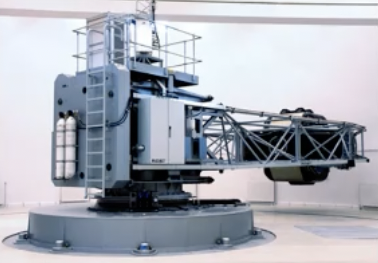
\includegraphics[width=0.25\textwidth]{problema_5.png}
\end{center}
\end{wrapfigure}

Una centrifugadora de entrenamiento de pilotos permite experimentar aceleraciones de 10*g (con $g=9.8\,m/s^2$). Si el brazo de la centrifugadora es de 8 m, calcula la velocidad lineal a la que hacen girar al piloto.\\

\textbf{Formulas base:}\\

Se tomarán las siguientes formulas base del MCUA:

\begin{align}
\boxed{ \vec{a_{c}} = \frac{v^2}{r} = \frac{(w \cdot r)^2}{r} = w^2 \cdot r}\\
\boxed{ a^2 + b^2 = c^2 }
\end{align}

\textbf{Solución:}\\

Es necesario poder descomponer la aceleración experimentada ($10 \cdot g$) en sus dos componentes o aceleraciones asociadas: aceleración centrípeta ($g = 9.8\,m/s$) y su aceleración tangencial (o centrífuga), que es finalmente la aceleración que se debe determinar. Dado que hablamos de un triangulo rectángulo, se puede aplicar la ecuación de pitágoras para su despeje, a saber:

\begin{align*}
\vec{a} &= 98\,m/s^2\\
\vec{a_{c}} &= 9.8\,m/s^2\\
\vec{a_{t}} &= ?
\end{align*}

Así que despejamos:

\begin{align*}
\vec{a^2} &= \vec{a_{c}^2} + \vec{a_{t}^2}\\
\vec{a_{t}} &= \sqrt{98^2 - 9.8^2}\\
\vec{a_{t}} &= 97.5088\,m/s^2
\end{align*}

Con el valor de la aceleración centrifuga determinado, procedemos a despejar la velocidad lineal, a saber:

\begin{align*}
\vec{a_{c}} &= \frac{v^2}{r}\\
v &= \sqrt{a_{c} \cdot r}\\
v &= \sqrt{97.5088 \cdot 8}\\
v &= 27.9297\,m/s
\end{align*}

De tal forma, que la velocidad lineal corresponde a $27.9297\,m/s \approx 27.93\,m/s$.

%%%%%%%%%%%%%%%%%%%%

\end{document}

